%%%%%%%%%%%%%%%%%%%%%%%%%%%%%%%%%%%%%%%%%%%%%%%%%%%%%%%%%%%%%%%%%%%%%%%%%%%%%%%%%%%%%%%%%%

% DIT MATERIAAL VERTROK VAN DE OPEN-SOURCE CURSUS VEELTERMEN VAN KOEN DE NAEGHEL         
% GEKOPIEËRD OP 24 MAART 2025                                                            
% ORIGINEEL BESCHIKBAAR VIA https://www.koendenaeghel.be/opensource.htm         

%%%%%%%%%%%%%%%%%%%%%%%%%%%%%%%%%%%%%%%%%%%%%%%%%%%%%%%%%%%%%%%%%%%%%%%%%%%%%%%%%%%%%%%%%%



\documentclass{ximera}

% vier voorkeuren die je meteen zelf kan instellen:
\def\uitbr{0} % waarde 1 als je Uitbreiding in de marge wilt, 0 als je dat niet wilt 
\def\wsg{0} % waarde 1 als je verwijzingen naar Wiskunde Samen gevat² in de marge wilt, 0 als je dat niet wilt
\def\rectoverso{0} % waarde 1 als je het PDF-bestand recto-verso wilt laten afdrukken, 0 als je het recto wilt
\def\voetn{1} % waarde 1 als je de voetnoten wilt, 0 als je dat niet wilt 

% marges:
\usepackage[paper=a4paper,margin=3.4cm,marginparwidth=2cm]{geometry}

% packages algemeen:
\pdfOnly{
\usepackage[english,dutch]{babel}
}
\usepackage{amsfonts}
\usepackage{amsmath} %  o.a. \eqref en \text, omgeving equation*
\usepackage{amssymb} % o.a. \nmid
\usepackage{amsthm} % o.a. omgeving proof
\usepackage{graphicx} % o.a. figuren
\usepackage{xcolor} % \color
\usepackage[disable]{todonotes} % \todo 
\usepackage{comment} % omgeving comment
\usepackage{xcolor} % kleuren 
\usepackage[skip=7pt plus1pt, indent=0pt]{parskip} % skip = verticale ruimte tussen twee alinea's, indent = insprong bij nieuwe alinea
\usepackage{multicol} % kolommen
\usepackage{xfrac} % breuken

\usepackage{siunitx} % SI eenheden
\usepackage{eso-pic} % achtergrond voorpagina
\usepackage{tabularx} % kolommen voor rekenmachine
\usepackage{rotating} % voor omgeving turn

% voor figuren met PSTricks:
\usepackage{pstricks} 
\usepackage{pstricks-add}
\usepackage{pst-plot}
\usepackage{pst-node}
\usepackage{pst-coil}
\usepackage{auto-pst-pdf}

% voor figuren met TikZ:
\usepackage{tikz} 
\usepackage{tkz-euclide} 
\usepackage{pgfplots} 
\usetikzlibrary{calc,intersections,through,backgrounds,patterns} 
\pgfplotsset{compat=newest}
\usepgfplotslibrary{fillbetween,colormaps}
\usepackage{import}
\usepackage{tikz-3dplot}

% zelfde parskip in minipage:
\makeatletter
\setlength{\parskip}{\medskipamount}
\newcommand{\@minipagerestore}{\setlength{\parskip}{\medskipamount}}
\makeatother

% voor veranderen van de naam Bibliografie naar Referentielijst:
\pdfOnly{
\addto\captionsdutch{\renewcommand{\bibname}{Referentielijst}}

% voor trefwoordenlijst:
\usepackage{imakeidx}
\makeindex[title=Trefwoordenlijst,program=makeindex,options=-s index.tex,columns=2,intoc=true]
}
% voor nummeren van vergelijkingen:
%WIM%\numberwithin{equation}{chapter} % als je dit desactiveert dan worden vergelijkingen in bijvoorbeeld hoofdstuk 3 genummerd als (1), (2) etc. in plaats van (3.1), (3.2) etc.

% voor hyperlinks en bladwijzers in PDF-bestand:
%WIM%\usepackage[bookmarksopen,bookmarksopenlevel=0,hypertexnames=false,pdfa,bookmarksnumbered]{hyperref} 
%WIM%\usepackage{bookmark} 

% voor hyperlinks: 
\hypersetup{pdfborder={0 0 0}, pdfstartpage=1,linkbordercolor={1 0 0}}%pdfborder={0 0 0} is geen rand rond hyperlinks, pdfborder={1 1 1} wel

% korter commando voor displaystyle, om bijvoorbeeld breuken groter te drukken in doorlopende tekst: 
\newcommand{\D}{\displaystyle}

% (veel)gebruikte verzamelingen:
\newcommand\NN{\mathbb{N}} % verzameling van de natuurlijke getallen
\newcommand\QQ{\mathbb{Q}} % verzameling van de rationale getallen
\newcommand\RR{\mathbb{R}} % verzameling van de re\"ele getallen
\newcommand\ZZ{\mathbb{Z}} % verzameling van de gehele getallen

% (veel)gebruikte operatoren:
\def\co{\operatorname{co}} % coördinaat van een punt
\def\ggd{\operatorname{ggd}} % positieve grootste gemene deler van twee gehele getallen niet beide nul
\def\gr{\operatorname{gr}} % graad van een veelterm

% voor kleur grafieken (donkergroen):
\definecolor{graf}{RGB}{0,100,0} 

% voor lijsten: 
% \usepackage{enumerate}
%WIM%\usepackage[shortlabels]{enumitem} 
\setlist{topsep=0em, itemsep=-0.15em}

% voor small bullet:
\newcommand\sbullet[1][.5]{\mathbin{\vcenter{\hbox{\scalebox{#1}{$\bullet$}}}}}

% voor meer verticale ruimte tussen vergelijkingen in align
\addtolength{\jot}{0.1cm}

% voor meervoudige voetnoten:
\usepackage{fnpct}

% voor het onderdrukken van voetnoten als optie:
\usepackage{letltxmacro}
\LetLtxMacro\Oldfootnote\footnote
\newcommand{\EnableFootNotes}{%
  \LetLtxMacro\footnote\Oldfootnote%
}
\newcommand{\DisableFootNotes}{%
  \renewcommand{\footnote}[2][]{\relax}
}

% voor verticale lijn in de marge (uitbreiding):
\usepackage[framemethod=default]{mdframed}
\usepackage{marginnote}
\reversemarginpar
\ifthenelse{\uitbr < 1}{\definecolor{rood}{RGB}{255,255,255}}{\definecolor{rood}{RGB}{254,64,64}} %HEX: #fe4040
\mdfdefinestyle{uitbreiding}{%
    topline=false,
    rightline=false,
    bottomline=false,
    leftline=true,
    linecolor=rood,
    linewidth=5pt,
    rightmargin=0pt,
    skipabove=10pt,% ipv 3
    skipbelow=0pt,
    leftmargin=-25pt,
    innerleftmargin=20pt,
    innerrightmargin=0pt,
    innertopmargin=0pt,
    innerbottommargin=0pt%,
%	needspace=30pt %minimumhoogte vooraleer lijn wordt gesplitst
    }
\newenvironment{Uitbreiding}{
    \marginpar{
        \center
		\vspace{0.1cm}
		\vspace{7pt}
		\rotatebox{90}{\color{rood}\Large \bf Uitbreiding}
	}
    \begin{mdframed}[style=uitbreiding]
    }{\vspace{-0.05cm}
    \end{mdframed}
}


% omgevingen voor lemma, definitie, voorbeeld etc.:
\newtheoremstyle{mystyle}
    {0em} % Space above
    {0em} % Space below
    {\itshape} % Body font
    {} % Indent amount
    {\bfseries} % Theorem head font
    {.} % Punctuation after theorem head
    {.5em} % Space after theorem head
    {} % Theorem head spec (can be left empty, meaning `normal')
\theoremstyle{mystyle}
%WIM%\newtheorem{lemma}{Lemma}[chapter] % als je [chapter] desactiveert dan Voorbeeld 3 in plaats van Voorbeeld 5.3, als je [chapter] vervangt door [section] dan Voorbeeld 5.2.3 in plaats van Voorbeeld 5.3 
%\theoremstyle{definition} % als je dit activeert dan is wat in de omgeving staat niet cursief gedrukt
\newtheorem{oefening}[lemma]{Oefening}
\newtheorem{definitie}[lemma]{Definitie} 
\newtheorem{voorbeeld}[lemma]{Voorbeeld}
\newtheorem{eigenschap}[lemma]{Eigenschap} 
\newtheorem{stelling}[lemma]{Stelling} 
\newtheorem{gevolg}[lemma]{Gevolg} 
\newtheorem{afspraak}[lemma]{Afspraak} 
\newtheorem{werkwijze}[lemma]{Werkwijze}

% omgeving proof, aangepaste ruimte: 
\makeatletter
\renewenvironment{proof}[1][\proofname]{\par
  \vspace{-\topsep}% remove the space after the theorem
  \pushQED{\qed}%
  \normalfont
  \topsep0pt \partopsep0pt % no space before
  \trivlist
  \item[\hskip\labelsep
        \itshape
    #1\@addpunct{.}]\ignorespaces
}{%
  \popQED\endtrivlist\@endpefalse
  \addvspace{0pt plus 0pt} % no space after
}
\makeatother

% kaderstijlen uit SOHO Wiskunde Plantyn:
\colorlet{steunkleur}{black}
\colorlet{steunkleurlicht}{steunkleur!30!white}
\colorlet{steunkleurkader}{steunkleur!7!white}
\colorlet{steunkleurkaderlicht}{steunkleur!2!white}

\mdfdefinestyle{kaderstijl_vol_licht}
{skipabove=6pt, 
skipbelow=6pt, 
backgroundcolor=steunkleurkader,
linecolor=steunkleurlicht,
linewidth = 0.4pt, 
topline=true,
bottomline=true, 
rightline=true,
innerleftmargin=5pt,
innerrightmargin=5pt,
innertopmargin=5pt,
leftmargin=0cm,
rightmargin=0cm,
innerbottommargin=5pt,
needspace=30pt % minimumhoogte voor splitsen kader
}
\surroundwithmdframed[style=kaderstijl_vol_licht]{definitie}
\surroundwithmdframed[style=kaderstijl_vol_licht]{stelling}
\surroundwithmdframed[style=kaderstijl_vol_licht]{lemma}
\surroundwithmdframed[style=kaderstijl_vol_licht]{eigenschap}
\surroundwithmdframed[style=kaderstijl_vol_licht]{gevolg}

% voor omgevingen voor oefening en antwoord:
\newenvironment{Oefening}{%
    \begin{enumerate}[ 
    series=Oef,
    resume=Oef,
    leftmargin=1.78em,
    label={\bfseries\arabic*.},
    ref=\arabic*
    ]
    \item %
    }{%
    \end{enumerate}
}
\newenvironment{Antwoord}{%
    \begin{enumerate}[%
    series=Antw,
    resume=Antw,
    leftmargin=1.78em,
    label={\bfseries\arabic*.},
    ref=\arabic*
    ]
    \item %
    }{%
    \end{enumerate}
}

% als de omgeving Uitbreiding start met een kaderomgeving (definitie, stelling, eigenschap, lemma of gevolg) dan moet wat extra verticale ruimte voorzien worden, met het commando \uitbreidingstartmetkader:
\def\uitbreidingstartmetkader{\mbox{}\vspace{-0.205cm}}

% % voor schema van de staartdeling:
% \usepackage{stackengine}
% \setstackgap{S}{5pt}
% \stackMath\def\stackalignment{r}
% \newcommand{\myRule}[3][white]{\textcolor{#1}{\rule{#2}{#3}}}
% \let\ph\phantom % enkel voor tekst
% \newcommand{\mph}[1]{% enkel voor math mode
%     \mathcolor{white}{#1}%
% }
% \def\staartmin{\rule{0.25cm}{0.1mm}\myRule{0.3cm}{0.1mm}}
% \def\staartphmin{\myRule{0.25cm}{0.1mm}\myRule{0.3cm}{0.1mm}}
% \newcommand{\staartstreep}[1]{\rule{\widthof{$#1$}}{0.1mm}}
% \newcommand{\staartphstreep}[1]{\myRule{\widthof{$#1$}}{0.1mm}}

% voor kolommen met schema van Horner:
\newcommand{\kolbreed}{1.0cm}
\newcolumntype{H}{>{\centering\arraybackslash$} p{\kolbreed} <{$}}

% voor nieuw commando utikzdashed: onderlijn (zoals underline) maar dan met stippellijn:
\tikzset{
    cheating dash/.code args={on #1 off #2 ends #3}{%
        \csname tikz@addoption\endcsname{%
            \pgfgetpath\currentpath%
            \pgfprocessround{\currentpath}{\currentpath}%
            \csname pgf@decorate@parsesoftpath\endcsname{\currentpath}{\currentpath}%
            \pgfmathparse{max(#1-#3,0)}\let\dashphase=\pgfmathresult%
            \pgfmathparse{\csname pgf@decorate@totalpathlength\endcsname-#1+2*\dashphase}\let\rest=\pgfmathresult%
            \pgfmathparse{#1+#2}\let\onoff=\pgfmathresult%
            \pgfmathparse{max(floor(\rest/\onoff), 1)}\let\nfullonoff=\pgfmathresult%
            \pgfmathparse{max((\rest-\onoff*\nfullonoff)/\nfullonoff+#2, #2)}\let\offexpand=\pgfmathresult%
            \pgfsetdash{{#1}{\offexpand}}{\dashphase pt}}%
    },
    cheating dash per segment/.style args={on #1 off #2 ends #3}{
        /utils/exec=\csname tikz@options\endcsname,%
        decoration={show path construction,
            lineto code={\draw [cheating dash=on #1 off #2 ends #3] (\tikzinputsegmentfirst) -- (\tikzinputsegmentlast);},
            curveto code={\draw [cheating dash=on #1 off #2 ends #3] (\tikzinputsegmentfirst) .. controls (\tikzinputsegmentsupporta) and (\tikzinputsegmentsupportb) .. (\tikzinputsegmentlast);},
            closepath code={\draw [cheating dash=on #1 off #2 ends #3] (\tikzinputsegmentfirst) -- (\tikzinputsegmentlast);}
        },
        decorate,
    },
}
\newcommand{\utikzdash}[1]{%
    \tikz[baseline=(todotted.base)]{
        \node[inner sep=0pt,outer sep=1.5pt] (todotted) {#1};
        \draw[cheating dash per segment=on 2pt off 2pt ends 2pt, line width=0.4pt] (todotted.south west) -- (todotted.south east);
    }%
}%

\providecommand{\xmemph}[1]{\textit{#1}}

% voor nieuw commando underdashed: onderlijn met stippellijnen en ook het woord cursief zetten:
\newcommand{\underdashed}[1]{%
    {\em\utikzdash{\!#1\!}}%
}

% voor icoon TI-84 Plus met verwijzing naar filmpje:
\newcommand{\grmlink}{\raisebox{0cm}{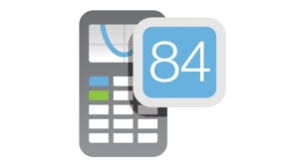
\includegraphics[width=1cm]{TI84Plus-icoon}}}
\newcommand{\grmref}[1]{%
	\reversemarginpar%
	\marginpar{
		\vspace{-0.4cm}%
		\htmladdnormallink{\grmlink}{#1}
	}	
}

% GRM knoppen:
\newcommand{\GRM}[1]{\fbox{\rule[0mm]{0cm}{0.215cm}\textup{\texttt{#1}}}}
\newcommand{\wedgetext}{{\raisebox{0.02cm}{\begin{turn}{90}>\end{turn}}}}
\newcommand{\veetext}{\raisebox{0.2cm}{\begin{turn}{-90}>\end{turn}}}

% voor kolommen met GRM screens:
\newlength{\widthallscreens}
\newlength{\widthscreens}
\newlength{\spaceleftscreen}
\newlength{\spacerightscreen}
\newlength{\spacebetweenscreens}

\newcommand{\setscreens}{
	\setlength{\spaceleftscreen}{2pt}
	\setlength{\spacerightscreen}{2pt}
	\setlength{\spacebetweenscreens}{8pt}
	\addtolength{\linewidth}{-28pt} % 3*8pt tussen vier screens en 2 pt links en 2 pt rechts
	\setlength{\widthallscreens}{\linewidth}
	\setlength{\widthscreens}{0.25\widthallscreens}
	\addtolength{\linewidth}{28pt}
	\newcolumntype{G}{p{\widthscreens}}
	\newcolumntype{s}{p{\spacebetweenscreens}}
	\newcolumntype{L}{p{\spaceleftscreen}}
	\newcolumntype{R}{p{\spacerightscreen}}
	\setlength{\tabcolsep}{0pt}
}

% voor icoon met verwijzing naar Wiskunde Samen gevat² in de marge:
% \newcommand{\wsglink}{\raisebox{0cm}{\includegraphics[width=1cm]{wsglogo}}}
\newcommand{\wsglink}{\raisebox{0cm}{LOGO}}
\newcommand{\htmladdnormallink}[2]{\href{#2}{#1}}
\newcounter{pagnrwsg}
\newcommand{\wsgref}[3]{% 
    % #1 woord dat onderstippeld wordt
    % #2 pagina van Wiskunde Samen gevat² waar je op terecht komt als je op de link klikt  
    % #3 afgedrukt op het logo van Wiskunde Samen gevat² in de marge: één of meerdere paginanummers
    \ifthenelse{\wsg < 1}{#1}{%
        \underdashed{#1}%
        {\setcounter{pagnrwsg}{#2}}%
        {\addtocounter{pagnrwsg}{14}}%
        \reversemarginpar%
        \marginpar{\vspace{-0.6cm}%
           \htmladdnormallink{\wsglink}{https://online.fliphtml5.com/sanky/laea/\#p=\arabic{pagnrwsg}}%
            \raisebox{0.41cm}[0cm][0cm]{%
                \hspace{-1.5cm}\makebox[2cm][c]{\colorbox{white}{\texttt{\footnotesize{#3}}}}%
            }%
        }%
    }%
}

% voor invoegen blanco pagina bij de optie recto-verso:
\def\blancobijrectoverso{
	\ifthenelse{\rectoverso < 1}{\clearpage}{
	\clearpage
	\thispagestyle{empty}
	\mbox{}
	\clearpage
	}
}

% aantal pagina's van het bestand:
\ifthenelse{\rectoverso < 1}{\def\totpag{57}}{\def\totpag{66}}

% documenteigenschappen:
% \usepackage{hyperxmp}
% \hypersetup{
% pdftitle={Open Source Wiskunde Aan zet: Veeltermen}, 
% pdfnumpages={\totpag},
% pdfauthor={Koen De Naeghel},
% pdflang={nl},
% pdfkeywords={wiskunde, open source, wiskunde aan zet, veeltermen, secundair onderwijs, tweede graad, doorstroomfinaliteit},
% pdfsubject={Veeltermen},
% pdfcopyright={\unichar{"24B8} 2024 Koen De Naeghel},
% pdfdate={17 december 2024},
% pdfapart=1,
% pdfstartview=}

% voor het benoemen van titel, auteur en datum:
% \title{Veeltermen}
% \author{Auteur: Koen De Naeghel}
% \date{\today}

\newcommand\BackgroundPic{
    \put(-260,-125){
    \parbox[b][\paperheight]{\paperwidth}{%
    \vfill
    \centering
    
\includegraphics[height=\paperwidth, keepaspectratio]{WaZlogo}%
    \vfill
}}}

% Laatste wijziging: 24/12/2024 12:23

% Compileren in Overleaf: Menu > Settings > Compiler: XeLaTeX
% Compileren in TeXstudio: F4
% \documentclass[titlepage,10pt,oneside]{book} 

% zes voorkeuren die je meteen zelf kan instellen:
\def\uitbr{0} % waarde 1 als je Uitbreiding in de marge wilt, 0 als je dat niet wilt 
\def\wsg{0} % waarde 1 als je verwijzingen naar Wiskunde Samen gevat² wilt, 0 als je dat niet wilt (onderstippelde woorden in de hoofdtekst en logo met paginanummer en hyperlink naar boekpagina in de marge)
\def\rectoverso{0} % waarde 1 als je het PDF-bestand recto-verso wilt laten afdrukken, 0 als je het recto wilt
\def\voetn{0} % waarde 1 als je de voetnoten wilt, 0 als je dat niet wilt 
\def\grm{0} % waarde 1 als je de schermafdrukken van TI-84 Plus wilt, 0 als je dat niet wilt
\def\grmlogo{0} % waarde 1 als je logo TI-84 Plus in de marge wilt, 0 als je dat niet wilt (met hyperlink naar filmpje) 

% marges:
% \usepackage[paper=a4paper,margin=3.4cm,marginparwidth=2cm]{geometry}

% packages algemeen:
% \usepackage[english,dutch]{babel}
\usepackage{amsfonts}
\usepackage{amsmath} %  o.a. \eqref en \text, omgeving equation*
\usepackage{amssymb} % o.a. \nmid
\usepackage{amsthm} % o.a. omgeving proof
\usepackage{graphicx} % o.a. figuren
\usepackage{xcolor} % \color
% \usepackage[disable]{todonotes} % \todo 
\usepackage{comment} % omgeving comment
\usepackage{xcolor} % kleuren 
\usepackage[skip=7pt plus1pt, indent=0pt]{parskip} % skip = verticale ruimte tussen twee alinea's, indent = insprong bij nieuwe alinea
\usepackage{multicol} % kolommen
\usepackage{xfrac} % breuken

\usepackage{siunitx} % SI eenheden
\usepackage{eso-pic} % achtergrond voorpagina
\usepackage{tabularx} % kolommen voor rekenmachine
\usepackage{rotating} % voor omgeving turn

% voor figuren met PSTricks:
\usepackage{pstricks} 
\usepackage{pstricks-add}
\usepackage{pst-plot}
\usepackage{pst-node}
\usepackage{pst-coil}
\pdfOnly{
\usepackage{auto-pst-pdf}
}


% voor figuren met TikZ:
\usepackage{tikz} 
\usepackage{tkz-euclide} 
\usepackage{pgfplots} 
\usetikzlibrary{calc,intersections,through,backgrounds,patterns} 
\pgfplotsset{compat=newest}
\usepgfplotslibrary{fillbetween,colormaps}
\usepackage{import}
\usepackage{tikz-3dplot}

% zelfde parskip in minipage:
\makeatletter
\setlength{\parskip}{\medskipamount}
\newcommand{\@minipagerestore}{\setlength{\parskip}{\medskipamount}}
\makeatother

% voor veranderen van de naam Bibliografie naar Referentielijst:
% \addto\captionsdutch{\renewcommand{\bibname}{Referentielijst}}

% voor trefwoordenlijst:
\usepackage{imakeidx}
\makeindex[title=Trefwoordenlijst,program=makeindex,options=-s index.tex,columns=2,intoc=true]

% voor nummeren van vergelijkingen:
% \numberwithin{equation}{chapter} % als je dit desactiveert dan worden vergelijkingen in bijvoorbeeld hoofdstuk 3 genummerd als (1), (2) etc. in plaats van (3.1), (3.2) etc.

% voor hyperlinks en bladwijzers in PDF-bestand:
% \usepackage[bookmarksopen,bookmarksopenlevel=0,hypertexnames=false,pdfa,bookmarksnumbered]{hyperref} 
\usepackage{bookmark} 

% voor hyperlinks: 
\hypersetup{pdfborder={0 0 0}, pdfstartpage=1,linkbordercolor={1 0 0}}%pdfborder={0 0 0} is geen rand rond hyperlinks, pdfborder={1 1 1} wel

% korter commando voor displaystyle, om bijvoorbeeld breuken groter te drukken in doorlopende tekst: 
\newcommand{\D}{\displaystyle}




% ------------------------------------------------------------------ VERZAMELINGEN 

% (veel)gebruikte verzamelingen:
\def\NN{\mathbb{N}} % verzameling van de natuurlijke getallen
\def\QQ{\mathbb{Q}} % verzameling van de rationale getallen
\def\RR{\mathbb{R}} % verzameling van de re\"ele getallen
\def\ZZ{\mathbb{Z}} % verzameling van de gehele getallen






% (veel)gebruikte operatoren:
\def\co{\operatorname{co}} % coördinaat van een punt
\def\ggd{\operatorname{ggd}} % positieve grootste gemene deler van twee gehele getallen niet beide nul
\def\gr{\operatorname{gr}} % graad van een veelterm

% voor kleur grafieken (donkergroen):
\definecolor{graf}{RGB}{0,100,0} 





% voor lijsten: 
% \usepackage{enumerate}
% \usepackage[shortlabels]{enumitem} 
\setlist{topsep=0em, itemsep=-0.15em}

% voor small bullet:
\newcommand\sbullet[1][.5]{\mathbin{\vcenter{\hbox{\scalebox{#1}{$\bullet$}}}}}

% voor meer verticale ruimte tussen vergelijkingen in align
\addtolength{\jot}{0.1cm}


% --------------------------------------------------------------------- VOETNOTEN 



% voor meervoudige voetnoten:
\usepackage{fnpct}

% voor het onderdrukken van voetnoten als optie:
\usepackage{letltxmacro}
\LetLtxMacro\Oldfootnote\footnote
\newcommand{\EnableFootNotes}{%
  \LetLtxMacro\footnote\Oldfootnote%
}
\newcommand{\DisableFootNotes}{%
  \renewcommand{\footnote}[2][]{\relax}
}




% ------------------------------------------------------------LAYOUT UITWEIDING 


% voor verticale lijn in de marge (uitbreiding):
\usepackage[framemethod=default]{mdframed}
\usepackage{marginnote}
\reversemarginpar
\ifthenelse{\uitbr < 1}{\definecolor{rood}{RGB}{255,255,255}}{\definecolor{rood}{RGB}{254,64,64}} %HEX: #fe4040
\mdfdefinestyle{uitbreiding}{%
    topline=false,
    rightline=false,
    bottomline=false,
    leftline=true,
    linecolor=rood,
    linewidth=5pt,
    rightmargin=0pt,
    skipabove=10pt,% ipv 3
    skipbelow=0pt,
    leftmargin=-25pt,
    innerleftmargin=20pt,
    innerrightmargin=0pt,
    innertopmargin=0pt,
    innerbottommargin=0pt%,
%	needspace=30pt %minimumhoogte vooraleer lijn wordt gesplitst
    }

% --------------------------------------------------------------------- ENVIRONMENTS DEFINIËREN 

\newenvironment{Uitbreiding}{
    \marginpar{
        \center
		\vspace{0.1cm}
		\vspace{7pt}
		\rotatebox{90}{\color{rood}\Large \bf Uitbreiding}
	}
    \begin{mdframed}[style=uitbreiding]
    }{\vspace{-0.05cm}
    \end{mdframed}
}


% omgevingen voor lemma, definitie, voorbeeld etc.:
\newtheoremstyle{mystyle}
    {0em} % Space above
    {0em} % Space below
    {\itshape} % Body font
    {} % Indent amount
    {\bfseries} % Theorem head font
    {.} % Punctuation after theorem head
    {.5em} % Space after theorem head
    {} % Theorem head spec (can be left empty, meaning `normal')
\theoremstyle{mystyle}
% \newtheorem{lemma}{Lemma}[chapter] % als je [chapter] desactiveert dan Voorbeeld 3 in plaats van Voorbeeld 5.3, als je [chapter] vervangt door [section] dan Voorbeeld 5.2.3 in plaats van Voorbeeld 5.3 
%\theoremstyle{definition} % als je dit activeert dan is wat in de omgeving staat niet cursief gedrukt
\newtheorem{oefening}[lemma]{Oefening}
\newtheorem{definitie}[lemma]{Definitie} 
\newtheorem{voorbeeld}[lemma]{Voorbeeld}
\newtheorem{eigenschap}[lemma]{Eigenschap} 
\newtheorem{stelling}[lemma]{Stelling} 
\newtheorem{gevolg}[lemma]{Gevolg} 
\newtheorem{afspraak}[lemma]{Afspraak} 
\newtheorem{werkwijze}[lemma]{Werkwijze}

% omgeving proof, aangepaste ruimte: 
\makeatletter
\renewenvironment{proof}[1][\proofname]{\par
  \vspace{-\topsep}% remove the space after the theorem
  \pushQED{\qed}%
  \normalfont
  \topsep0pt \partopsep0pt % no space before
  \trivlist
  \item[\hskip\labelsep
        \itshape
    #1\@addpunct{.}]\ignorespaces
}{%
  \popQED\endtrivlist\@endpefalse
  \addvspace{0pt plus 0pt} % no space after
}
\makeatother

% kaderstijlen uit SOHO Wiskunde Plantyn:
\colorlet{steunkleur}{black}
\colorlet{steunkleurlicht}{steunkleur!30!white}
\colorlet{steunkleurkader}{steunkleur!7!white}
\colorlet{steunkleurkaderlicht}{steunkleur!2!white}

\mdfdefinestyle{kaderstijl_vol_licht}
{skipabove=6pt, 
skipbelow=6pt, 
backgroundcolor=steunkleurkader,
linecolor=steunkleurlicht,
linewidth = 0.4pt, 
topline=true,
bottomline=true, 
rightline=true,
innerleftmargin=5pt,
innerrightmargin=5pt,
innertopmargin=5pt,
leftmargin=0cm,
rightmargin=0cm,
innerbottommargin=5pt,
needspace=30pt % minimumhoogte voor splitsen kader
}
\surroundwithmdframed[style=kaderstijl_vol_licht]{definitie}
\surroundwithmdframed[style=kaderstijl_vol_licht]{stelling}
\surroundwithmdframed[style=kaderstijl_vol_licht]{lemma}
\surroundwithmdframed[style=kaderstijl_vol_licht]{eigenschap}
\surroundwithmdframed[style=kaderstijl_vol_licht]{gevolg}

% voor omgevingen voor oefening en antwoord:
\newenvironment{Oefening}{%
    \begin{enumerate}[ 
    series=Oef,
    resume=Oef,
    leftmargin=1.78em,
    label={\bfseries\arabic*.},
    ref=\arabic*
    ]
    \item %
    }{%
    \end{enumerate}
}
\newenvironment{Antwoord}{%
    \begin{enumerate}[%
    series=Antw,
    resume=Antw,
    leftmargin=1.78em,
    label={\bfseries\arabic*.},
    ref=\arabic*
    ]
    \item %
    }{%
    \end{enumerate}
}

% --------------------------------------------------------------------- 




% als de omgeving Uitbreiding start met een kaderomgeving (definitie, stelling, eigenschap, lemma of gevolg) dan moet wat extra verticale ruimte voorzien worden, met het commando \uitbreidingstartmetkader:
\def\uitbreidingstartmetkader{\mbox{}\vspace{-0.205cm}}

% ---------------------------------------------------------------------  voor schema van de staartdeling:
\usepackage{stackengine}
\setstackgap{S}{5pt}
\stackMath\def\stackalignment{r}
\newcommand{\myRule}[3][white]{\textcolor{#1}{\rule{#2}{#3}}}
\let\ph\phantom % enkel voor tekst
\newcommand{\mph}[1]{% enkel voor math mode
    \mathcolor{white}{#1}%
}
\def\staartmin{\rule{0.25cm}{0.1mm}\myRule{0.3cm}{0.1mm}}
\def\staartphmin{\myRule{0.25cm}{0.1mm}\myRule{0.3cm}{0.1mm}}
\newcommand{\staartstreep}[1]{\rule{\widthof{$#1$}}{0.1mm}}
\newcommand{\staartphstreep}[1]{\myRule{\widthof{$#1$}}{0.1mm}}





% voor kolommen met schema van Horner:
\newcommand{\kolbreed}{1.0cm}
\newcolumntype{H}{>{\centering\arraybackslash$} p{\kolbreed} <{$}}



% --------------------------------------------------------------------- HEEL DIT UNDERDASHED KAN WEG DENKIK 


% voor nieuw commando utikzdashed: onderlijn (zoals underline) maar dan met stippellijn:
\tikzset{
    cheating dash/.code args={on #1 off #2 ends #3}{%
        \csname tikz@addoption\endcsname{%
            \pgfgetpath\currentpath%
            \pgfprocessround{\currentpath}{\currentpath}%
            \csname pgf@decorate@parsesoftpath\endcsname{\currentpath}{\currentpath}%
            \pgfmathparse{max(#1-#3,0)}\let\dashphase=\pgfmathresult%
            \pgfmathparse{\csname pgf@decorate@totalpathlength\endcsname-#1+2*\dashphase}\let\rest=\pgfmathresult%
            \pgfmathparse{#1+#2}\let\onoff=\pgfmathresult%
            \pgfmathparse{max(floor(\rest/\onoff), 1)}\let\nfullonoff=\pgfmathresult%
            \pgfmathparse{max((\rest-\onoff*\nfullonoff)/\nfullonoff+#2, #2)}\let\offexpand=\pgfmathresult%
            \pgfsetdash{{#1}{\offexpand}}{\dashphase pt}}%
    },
    cheating dash per segment/.style args={on #1 off #2 ends #3}{
        /utils/exec=\csname tikz@options\endcsname,%
        decoration={show path construction,
            lineto code={\draw [cheating dash=on #1 off #2 ends #3] (\tikzinputsegmentfirst) -- (\tikzinputsegmentlast);},
            curveto code={\draw [cheating dash=on #1 off #2 ends #3] (\tikzinputsegmentfirst) .. controls (\tikzinputsegmentsupporta) and (\tikzinputsegmentsupportb) .. (\tikzinputsegmentlast);},
            closepath code={\draw [cheating dash=on #1 off #2 ends #3] (\tikzinputsegmentfirst) -- (\tikzinputsegmentlast);}
        },
        decorate,
    },
}
\newcommand{\utikzdash}[1]{%
    \tikz[baseline=(todotted.base)]{
        \node[inner sep=0pt,outer sep=1.5pt] (todotted) {#1};
        \draw[cheating dash per segment=on 2pt off 2pt ends 2pt, line width=0.4pt] (todotted.south west) -- (todotted.south east);
    }%
}%

% voor nieuw commando underdashed: onderlijn met stippellijnen en ook het woord cursief zetten:
\newcommand{\underdashed}[1]{%
    {\em\utikzdash{\!#1\!}}%
}



% ----------------------------------------------------------hier doet koen allemaal GRM 

% voor icoon TI-84 Plus met verwijzing naar filmpje:
\newcommand{\grmlink}{\raisebox{0cm}{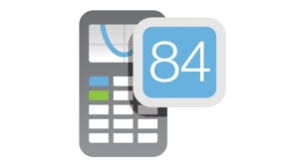
\includegraphics[width=1cm]{TI84Plus-icoon}}}
\newcommand{\grmref}[1]{%
	\ifthenelse{\grmlogo < 1}{}{
		\reversemarginpar%
		\marginpar{
			\vspace{-0.4cm}%
			\htmladdnormallink{\grmlink}{#1}
		}
	}	
}




% GRM knoppen:
\newcommand{\GRM}[1]{\fbox{\rule[0mm]{0cm}{0.215cm}\textup{\texttt{#1}}}}
\newcommand{\wedgetext}{{\raisebox{0.02cm}{\begin{turn}{90}>\end{turn}}}}
\newcommand{\veetext}{\raisebox{0.2cm}{\begin{turn}{-90}>\end{turn}}}




% voor kolommen met GRM screens:
\newlength{\widthallscreens}
\newlength{\widthscreens}
\newlength{\spaceleftscreen}
\newlength{\spacerightscreen}
\newlength{\spacebetweenscreens}




\newcommand{\setscreens}{
	\setlength{\spaceleftscreen}{2pt}
	\setlength{\spacerightscreen}{2pt}
	\setlength{\spacebetweenscreens}{8pt}
	\addtolength{\linewidth}{-28pt} % 3*8pt tussen vier screens en 2 pt links en 2 pt rechts
	\setlength{\widthallscreens}{\linewidth}
	\setlength{\widthscreens}{0.25\widthallscreens}
	\addtolength{\linewidth}{28pt}
	\newcolumntype{G}{p{\widthscreens}}
	\newcolumntype{s}{p{\spacebetweenscreens}}
	\newcolumntype{L}{p{\spaceleftscreen}}
	\newcolumntype{R}{p{\spacerightscreen}}
	\setlength{\tabcolsep}{0pt}
}





% -------------------------------------------------------------------------ICOON IN DE MARGE 

% voor icoon met verwijzing naar Wiskunde Samen gevat² in de marge:
\newcommand{\wsglink}{\raisebox{0cm}{\includegraphics[width=1cm]{wsglogo}}}
\newcommand{\htmladdnormallink}[2]{\href{#2}{#1}}
\newcounter{pagnrwsg}
\newcommand{\wsgref}[3]{% 
    % #1 woord dat onderstippeld wordt
    % #2 pagina van Wiskunde Samen gevat² waar je op terecht komt als je op de link klikt  
    % #3 afgedrukt op het logo van Wiskunde Samen gevat² in de marge: één of meerdere paginanummers
    \ifthenelse{\wsg < 1}{#1}{%
        \underdashed{#1}%
        {\setcounter{pagnrwsg}{#2}}%
        {\addtocounter{pagnrwsg}{14}}%
        \reversemarginpar%
        \marginpar{\vspace{-0.6cm}%
           \htmladdnormallink{\wsglink}{https://online.fliphtml5.com/sanky/laea/\#p=\arabic{pagnrwsg}}%
            \raisebox{0.41cm}[0cm][0cm]{%
                \hspace{-1.5cm}\makebox[2cm][c]{\colorbox{white}{\texttt{\footnotesize{#3}}}}%
            }%
        }%
    }%
}





% -----------------------------------------NICE TO HAVES 

% voor invoegen blanco pagina bij de optie recto-verso:
\def\blancobijrectoverso{
	\ifthenelse{\rectoverso < 1}{\clearpage}{
	\clearpage
	\thispagestyle{empty}
	\mbox{}
	\clearpage
	}
}

% aantal pagina's van het bestand:
\ifthenelse{\rectoverso < 1}{\def\totpag{57}}{\def\totpag{66}}



% documenteigenschappen:
\usepackage{hyperxmp}
\hypersetup{
pdftitle={Open Source Wiskunde Aan zet: Veeltermen}, 
pdfnumpages={\totpag},
pdfauthor={Koen De Naeghel},
pdflang={nl},
pdfkeywords={wiskunde, open source, wiskunde aan zet, veeltermen, secundair onderwijs, tweede graad, doorstroomfinaliteit},
pdfsubject={Veeltermen},
pdfcopyright={\unichar{"24B8} 2024 Koen De Naeghel},
pdfdate={17 december 2024},
pdfapart=1,
pdfstartview=}

% voor het benoemen van titel, auteur en datum:
\title{Veeltermen}
\author{Auteur: Koen De Naeghel}
\date{\today}

\newcommand\BackgroundPic{
    \put(-260,-125){
    \parbox[b][\paperheight]{\paperwidth}{%
    \vfill
    \centering
    
\includegraphics[height=\paperwidth, keepaspectratio]{WaZlogo}%
    \vfill
}}}

\addPrintStyle{..}
\begin{document}
\author{Koen de Naeghel - Wiskunde Op Maat}
\xmtitle{Veeltermen}{}



\section{Veeltermen}

Als $ax^n$ en $bx^m$ eentermen zijn, dan kunnen we de uitdrukking $ax^n + bx^m$ bekijken, die we opvatten als de {\em som} van die twee eentermen. Het resultaat noemen we een {\em tweeterm}. Analoog kunnen we spreken over een {\em drieterm}, een {\em vierterm} enzovoort. Algemeen spreken we dan van een {\em veelterm}.

\begin{definition} 
Een \underline{(re\"ele) veelterm in (de variabele) $x$}\index{veelterm} is een eindige som van eentermen in $x$.
\end{definition} 

\begin{example} 
De volgende uitdrukkingen zijn veeltermen in $x$:
\[
3x^2, \qquad \sqrt{5} - 8x, \qquad -1 + 3x -2x^2 \qquad \text{ en } \qquad -\frac{4}{3}x^5 - 2x^3 + \pi^2\,x + 5. 
\]
\end{example} 

We willen nu ook een willekeurige veelterm in symbolen kunnen schrijven. Als de graad van de eentermen die voorkomen niet te hoog is, kan dat als volgt:
\begin{align*} 
\left\{
\begin{aligned}
& a && \text{ waarbij } a \in \R  \\
& a + bx && \text{ waarbij } a,b \in \R  \\
& a + bx + cx^2 && \text{ waarbij } a,b,c \in \R  \\
& a + bx + cx^2 + dx^3 && \text{ waarbij } a,b,c,d \in \R \\
& \text{etc.} && 
\end{aligned}
\right.
\end{align*}
Van zodra er een eenterm van graad $26$ voorkomt, hebben we onvoldoende letters in het Latijns alfabet. Dat probleem kunnen we omzeilen door gebruik te maken van een {\em onderindex}\:: in plaats van $a,b,c$ etc. schrijven we $a_0, a_1, a_2$ etc. Op die manier kunnen we een willekeurige veelterm in symbolen uitdrukken.

\begin{definition} 
Een \underline{(re\"ele) veelterm in (de variabele) $x$}\index{veelterm} is een uitdrukking van de vorm $A(x) = a_0 + a_1x + a_2x^2 + \dots + a_n x^n$ waarbij $n \in \N$ en $a_0,a_1,a_2,\ldots,a_n \in \R$.
\end{definition} 

Spreken we in het vervolg van {\em een veelterm} $a_0 + a_1x + a_2x^2 + \dots + a_n x^n$ of $b_0 + b_1x + \dots + b_m x^m$ dan nemen we steeds aan dat $n,m\in \N$ en $a_0, \ldots, a_n\in \R$ en $b_0, \ldots, b_m\in \R$.

\begin{example} 
Kiezen we in de bovenstaande definitie $n = 4$ en $a_0 = -5$, $a_1 = 7$, $a_2 = -3$, $a_3 = 0$ en $a_4 = 0$ dan verkrijgen we de veelterm
\begin{align*}
A(x) 
& = a_0 + a_1x + a_2x^2 + \dots + a_n x^n \\
& = a_0 + a_1x + a_2x^2 + a_3 x^3 + a_4 x^4 \\ 
& = -5 + 7x - 3x^2 + 0x^3 + 0x^4 \\
& = -5 + 7x - 3x^2.
\end{align*}
We konden dus even goed $n = 2$ en $a_0 = -5$, $a_1 = 7$ en $a_2 = -3$ gekozen hebben. 
\end{example} 

Dankzij de afspraak $x^0 = 1$ kunnen we een veelterm herschrijven met het sommatieteken:
\[
A(x) = a_0 + a_1x + a_2x^2 + \dots + a_n x^n = \sum_{i=0}^n a_i x^i.
\]

\begin{example} 
Beschouw de veeltermen
\[
A(x) = \sum_{i=0}^3 (2i+1) x^i \qquad \text{ en } \qquad P(t) = \sum_{i=1}^5 \frac{1}{i^2} \, t^i.
\] 
Dan kunnen we die veeltermen uitschrijven als
\begin{align*}
A(x)  = (2\cdot0+1)x^0 + (2\cdot1+1)x^1 + (2\cdot2+1)x^2 + (2\cdot3+1)x^3 = 1 + 3x + 5x^2 + 7x^3
\end{align*}
en
\begin{align*}
P(x) 
& = \frac{1}{1^2} \, t^1 + \frac{1}{2^2} \, t^2 + \frac{1}{3^2} \, t^3 + \frac{1}{4^2} \, t^4 + \frac{1}{5^2} \, t^5 \\
& = t + \frac{1}{4}\,t^2 + \frac{1}{9}\,t^3 + \frac{1}{16}\,t^4 + \frac{1}{5}\,t^5.
\end{align*}
\end{example} 

Als $a_0 + a_1x + a_2x^2 + \dots + a_n x^n$ een veelterm is, dan noemen we de getallen $a_0, a_1, a_2, \ldots, a_n$ de \underline{co\"effici\"enten}\index{co\"effici\"ent}\index{veelterm!co\"effici\"enten} van de veelterm. De (een)termen $a_0, a_1x, a_2x^2, \ldots , a_nx^n$ noemen we de \underline{(een)termen} van de veelterm. De term $a_0$ wordt de \underline{constante term}\index{constante term}\index{veelterm!constante term} van de veelterm genoemd.

\begin{example} 
De constante term van de veelterm $A(x) = -5 + 7x - 3x^2$ is gelijk aan $-5$.  
\end{example} 

Als $a_0 + a_1x + a_2x^2 + \dots + a_n x^n$ een veelterm is waarbij $a_n \neq 0$, dan noemen we $n$ de \underline{graad}\index{graad}\index{veelterm!graad} van de veelterm. Schrijven we de veelterm als $A(x)$, dan noteren we de graad als $\gr A(x)$. In dat geval is $a_nx^n$ de \underline{hoogstegraadsterm}\index{hoogstegraadsterm}\index{veelterm!hoogstegraadsterm} en $a_n$ de \underline{hoogstegraadsco\"effici\"ent}\index{hoogstegraadsco\"effici\"ent}\index{veelterm!hoogstegraadsco\"effici\"ent} van de veelterm. De graad van de veelterm $0 + 0\cdot x + 0 \cdot x^2 + \dots + 0\cdot x^n = 0$ wordt in het secundair onderwijs niet gedefini\"eerd.

Veeltermen van graad nul, \'e\'en, twee of drie wordt respectievelijk \underline{constante}, \underline{lineaire}, \linebreak \underline{kwadratische} en \underline{kubische veeltermen} genoemd. Ook veelterm $0 + 0\cdot x + 0 \cdot x^2 + \dots + 0\cdot x^n = 0$ wordt een constante veelterm genoemd.

\begin{example} 
We vereenvoudigen onderstaande veeltermen, en geven telkens de graad, de hoogstegraadsco\"effici\"ent en constante term.
\begin{enumerate}[(a)]
\item
$A(x) = 1-4x+5x^3-7x^3 = 1 - 4x - 2x^3$ heeft graad $3$, hoogstegraadsco\"effici\"ent $-2$ en constante term $1$.
\item
$B(x) = 0x^2 + 3x = 3x$ heeft graad $1$, hoogstegraadsco\"effici\"ent $3$ en constante term $0$.
\item
$C(x) = \sqrt{7}-\sqrt{28} = \sqrt{7}-2\sqrt{7} = -\sqrt{7}$ heeft graad $0$, hoogstegraadsco\"effici\"ent $-\sqrt{7}$ en constante term $-\sqrt{7}$.
\end{enumerate}
\end{example} 

De verzameling van alle veeltermen in $x$ wordt genoteerd met $\R[x]$. In symbolen:
\[
\R[x] = \{a_0 + a_1 x + a_2 x^2 + \dots + a_n x^n \mid \text{$n \in \N$ en $a_0,a_1,a_2,\ldots,a_n \in \R$} \}.
\]
Wegens een eerdere afspraak is $a = a\cdot x^0$, zodat elk re\"eel getal $a$ kan geschreven worden als een veelterm. De verzameling van de re\"ele getallen is dus een deelverzameling
van de verzameling van alle veeltermen, in symbolen: $\R \subseteq \R[x]$. 

\begin{example} 
We hebben dat $1-4x+2x^3 \in \R[x]$, $x^5-\sqrt{2} \in \R[x]$ en $\D -\frac{13}{7} \in \R[x]$.   
\end{example} 

Twee veeltermen in $x$ zijn \underline{gelijk} als ze ofwel dezelfde graad en dezelfde co\"effici\"enten hebben, ofwel beide gelijk zijn aan nul. 

Soms komen er in wiskundige uitdrukkingen symbolen zoals $a$, $b$, $p$, $q$ etc. voor die getallen voorstellen. Pas als die symbolen een waarde toegekend krijgen, wordt de uitdrukking volledig vastgelegd. Zo'n symbool noemen we dan een {\em parameter}.\index{parameter} 

\begin{example} 
Beschouw $A(x) = ax^5 - 4x^2 + bx + 2$ en $B(x) = 7x^m + 2ax - c^2x^2 - d$ waarbij $a,b,c,d \in \R$ en $m \in \N$. We bepalen de waarde(n) van de parameters $a,b,c,d$ en $m$ waarvoor de veelterm $A(x)$ gelijk is aan de veelterm $B(x)$. We hebben: 
\begin{align*}
A(x) = B(x) \quad 
& \Leftrightarrow \quad ax^5 - 4x^2 + bx + 2 = 7x^m + 2ax - c^2x^2 - d \\
& \Leftrightarrow \quad 5 = m \,\,\text{ en }\,\, a = 7 \,\,\text{ en }\,\, -4 = -c^2 \,\,\text{ en }\,\, b = 2a \,\,\text{ en }\,\, 2 = -d \\
& \Leftrightarrow \quad m=5 \,\,\text{ en }\,\, a = 7 \,\,\text{ en }\,\, c^2 = 4 \,\,\text{ en }\,\, b = 14 \text{ en } d = -2 \\
& \Leftrightarrow \quad 
\left\{
\begin{aligned}
& m=5 \,\,\text{ en }\,\, a = 7 \,\,\text{ en }\,\, c = 2 \,\,\text{ en }\,\, b = 14 \text{ en } d = -2 \\
& \text{of} \\
& m=5 \,\,\text{ en }\,\, a = 7 \,\,\text{ en }\,\, c = -2 \,\,\text{ en }\,\, b = 14 \text{ en } d = -2.
\end{aligned}
\right.
\end{align*}
\end{example} 

Vervangen we in een veelterm $A(x)$ de variabele $x$ door een re\"eel getal $r$, dan verkrijgen we de \underline{getalwaarde}\index{veelterm!getalwaarde} van $A(x)$ in $x = r$. Die getalwaarde noteren we met $A(r)$. In symbolen:
\[
A(x) = a_0 + a_1x + a_2x^2 + \dots + a_n x^n \quad 
\Rightarrow
\quad A(r) = a_0 + a_1 r + a_2r^2 + \dots + a_n r^n
\]
met $n \in \N$ en $r, a_0, a_1, \ldots, a_n \in \R$, waarbij we ook hier het geval $n = r = 0$ uitsluiten. % voor ons heeft $0^0$ geen betekenis.

\begin{example} 
Als $A(x) = 2x^3+3x-5$ dan is de getalwaarde van $A(x)$ in $x = 10$ gelijk aan $A(10) = 2\cdot 10^3 + 3 \cdot 10 - 5 = 2025$.
\end{example} 

Is de getalwaarde van een veelterm in een re\"eel getal $r$ gelijk aan nul, dan noemen we $r$ een \underline{nulwaarde}\index{veelterm!nulwaarde} \index{nulwaarde} van die veelterm. De uitspraak {\em $r$ is een nulwaarde van $A(x)$} is dus gelijkwaardig met de uitspraak {\em $A(r) = 0$}. Met behulp van het symbool $\Leftrightarrow$ voor equivalentie wordt dit in symbolen:
\[
r \text{ is een nulwaarde van } A(x) \quad \Leftrightarrow \quad A(r) = 0.
\]
Hierbij is $r \in \R$ en $A(x)$ een veelterm in $x$. In de literatuur wordt een nulwaarde soms ook een \underline{nulpunt}\index{nulpunt} genoemd. Onze voorkeur gaat uit naar de volgende afspraak: een nulpunt is een punt (dus een meetkundig object), een nulwaarde is een waarde (dus een getal).

Bepalen van de waarde(n) van parameters kan leiden tot een stelsel. 
In het derde jaar heb je geleerd hoe je een stelsel van twee vergelijkingen in twee onbekenden kan oplossen. Die technieken moet je nog steeds kunnen toepassen. 

\begin{example} 
We bepalen de waarde(n) van de parameters $a$ en $b$ waarvoor
\[
a(x-3) - b(x+1) = 1-3x.
\]
We hebben:
\begin{align*}
a(x-3) - b(x+1) = 1-3x \quad 
& \Leftrightarrow \quad ax-3a-bx-b=1-3x \\
& \Leftrightarrow \quad (a-b)x +(-3a-b) = 1-3x \\
& \Leftrightarrow \quad
\left\{
\begin{aligned}
a - b & = -3 && (1)\\
-3a - b & = 1. && (2)
\end{aligned}
\right.
\end{align*}
Uit $(1)-(2)$ volgt $4a = -4$ zodat $a = -1$. Invullen in $(2)$ geeft $-1-b =  -3$ waaruit $b = 2$. 
\end{example} 

Bij een rekenoefening kan gevraagd worden om de berekening {\em algebra\"isch} uit te voeren: met de hand, waarbij je jouw tussenstappen met berekeningen opschrijft. Als het resultaat een re\"eel getal is, dan kan gevraagd worden om een exacte waarde te geven. Je kan uiteraard wel de rekenmachine gebruiken om jouw oplossing te controleren. 

Bij het algebra\"isch rekenwerk is het ook de bedoeling om het resultaat te vereenvoudigen. Je moet dus vlot kunnen rekenen met vierkantswortels en derdemachtswortels. 
Indien gevraagd maak je ook de noemers (vierkants)wortelvrij. 

\begin{example} 
Gegeven zijn de veeltermen
\[
A(x) = \frac{1}{5}\,x^2-3x+\frac{2}{3}, \quad B(x) = 3(bx)^2-6x+1 \quad \text{ en } \quad C(x) = x^3 + \sqrt[3]{2} x^2 + \sqrt[3]{4}x+5
\]
waarbij $b \in \R$. Hieronder voeren we het rekenwerk algebra\"isch uit, en geven telkens de exacte waarde van het eindresultaat. 
\begin{enumerate}[(a)]
\item
De getalwaarde van de veelterm $A(x)$ in $x = -2$ is gelijk aan
\[
A(-2) = \frac{1}{5}\,\cdot (-2)^2-3\cdot(-2)+\frac{2}{3} = \frac{4}{5} +6+ \frac{2}{3} = \frac{12 + 90 + 10}{15} = \frac{112}{15}.
\]
\item
We bepalen de waarde (n) van de parameter $b$ waarvoor $B(4) = 6$. We hebben:
\begin{align*}
B(4) = 6 \quad 
& \Leftrightarrow \quad 3(b\cdot 4)^2-6\cdot 4+1 = 6 \\ 
& \Leftrightarrow \quad 48b^2 = 29 \\
& \Leftrightarrow \quad b = \sqrt{\frac{29}{48}} \,\,\text{ of }\,\, b = - \sqrt{\frac{29}{48}} \\
& \Leftrightarrow \quad b = \frac{\sqrt{29}}{4\sqrt{3}} \,\,\text{ of }\,\, b = - \frac{\sqrt{29}}{4\sqrt{3}}
\end{align*}
\item
De getalwaarde van de veelterm $C(x)$ in $x = \sqrt[3]{2}$ is gelijk aan
\begin{align*}
C(\sqrt[3]{2}) & = (\sqrt[3]{2})^3 + \sqrt[3]{2}\cdot(\sqrt[3]{2})^2 + \sqrt[3]{4}\cdot \sqrt[3]{2}+5 \\
& = 2 + (\sqrt[3]{2})^3 + \sqrt[3]{2^2}\cdot \sqrt[3]{2} + 5 \\
& = 2 + 2 + (\sqrt[3]{2})^2 \cdot \sqrt[3]{2} + 5 \\
& = 2 + 2 + 2 + 5 \\
& = 11.
\end{align*}
\end{enumerate}
\end{example} 

De som van twee veeltermen in $x$ is opnieuw een veelterm in $x$. Ook het product van twee veeltermen in $x$ is opnieuw een veelterm in $x$. 

\begin{example} 
De som van $A(x) = 3x^3+2x^2-x+4$ met $B(x) = 6x^3-x^2+2$ is 
\[
A(x) + B(x) = 3x^3+2x^2-x+4 + 6x^3-x^2+2 = 9x^3 + x^2 - x + 6.
\]
Voor $P(x) = 6x^2-x+2$ en $Q(x) = -3x^3+5x^2$ is het product gelijk aan
\begin{align*}
P(x) \cdot Q(x) 
& = (6x^2-x+2) \cdot (-3x^3+5x^2) \\
& = 6x^2 \cdot (-3x^3) + 6x^2\cdot 5x^2 - x \cdot(-3x^3) - x \cdot 5x^2 + 2 \cdot(-3x^3) + 2 \cdot 5x^2 \\
& = -18x^5 + 30x^4 + 3x^4 - 5x^3 - 6x^3 + 10x^2 \\
& = -18x^5 + 33x^4 - 11x^3 + 10x^2.
\end{align*}
\end{example} 

In het voorbeeld hierboven is de graad van het product $P(x) \cdot Q(x)$ bepaald wordt door de graad van de hoogstegraadsterm $6x^2 \cdot (-3x^3) = -18 x^{5}$. We stellen dus vast dat de graad van het product gelijk is aan de som van de graden. Dat kenmerk geldt ook in het algemeen, in symbolen: 
\begin{equation} \label{eq:graadproduct}
\gr\bigl( A(x) \cdot B(x) \bigr) \, = \, \gr A(x) + \gr B(x)
\end{equation}
waarbij $A(x)$ en $B(x)$ veeltermen zijn, beide verschillend van de nulveelterm. 

In sommmige gevallen is de graad van de som van twee veeltermen gelijk aan het maximum van de graden van die twee veeltermen. Dat is bijvoorbeeld het geval met 
$A(x) = x^3$ en $B(x) = x^5 + 2x^2$. Inderdaad, dan is $A(x) + B(x) = x^5 + x^3 + 2x^2$ zodat $\gr\left(A(x) + B(x)\right) = 5$ gelijk is aan het maximum van de getallen $\gr A(x) = 3$ en $\gr B(x) = 5$. %In symbolen: $5 = \max\{3,5\}$. 

In andere gevallen kan het voorkomen dat de graad van de som van twee veeltermen kleiner is dan de graad van elk van die twee veeltermen. Dat is precies het geval wanneer de hoogste\-graadstermen van die twee veeltermen elkaars tegengestelde zijn. Zo is voor $A(x) = x^3$ en $C(x) = -x^3 + 2x^2$ de som gelijk aan $A(x) + C(x) = 2x^2$, waarvan de graad kleiner is dan $\max\{3,3\} = 3$. In het algemeen hebben we dat  
\begin{equation} \label{eq:graadsomenverschil}
\gr\bigl( A(x) \pm B(x) \bigr) \, \leq \, \max \bigl\{ \,\gr A(x)\, , \, \gr B(x) \, \bigr\}
\end{equation}
voor alle veeltermen $A(x)$ en $B(x)$ die beide verschillend zijn van de nulveelterm. In het geval dat $\gr A(x) \neq \gr B(x)$ dan geldt in de bovenstaande formule \eqref{eq:graadsomenverschil} steeds de gelijkheid. 

\begin{Uitbreiding}
Spreken we af dat $\gr 0 = - \infty$, dan zijn \eqref{eq:graadproduct} en \eqref{eq:graadsomenverschil} ook geldig voor het geval dat $A(x) = 0$ of $B(x) = 0$, zie Oefening \ref{oefgraadnulveelterm}. Vermeldenswaardig is de gelijkaardige uitdrukking voor de graad van de substitutie van een veelterm in een veelterm, die eenvoudig wordt aangetoond:
\[
\gr\Bigl(A\bigl(B(x\bigr)\Bigr) = \gr A(x) \cdot \gr B(x).
\]
\end{Uitbreiding}

\begin{example} 
Van drie veeltermen $A(x)$, $B(x)$ en $C(x)$ weten we dat
\[
\gr A(x) = 6, \quad \gr B(x) = 4 \quad \text{ en } \quad \gr C(x) = 1.
\]
We bepalen de graad van de veelterm $D(x) = A(x) - \bigl(B(x) + 2C(x)\bigr)$ door de bovenstaande formules \eqref{eq:graadproduct} en \eqref{eq:graadsomenverschil} toe te passen. 

Vooreerst is $\gr\bigl(2C(x)\bigr) = \gr(2) + \gr C(x) = 0 + 1 = 1$. Nu is $\gr B(x) \neq \gr\bigl(2C(x)\bigr)$ zodat
\[
\gr \bigl(B(x) + 2C(x)\bigr) = \max \bigl\{\gr B(x),\gr\bigl(2C(x)\bigr)\bigr\} = \max\{4,1\} = 4.
\]
Verder is $\gr A(x) \neq \gr\bigl(B(x) + 2C(x)\bigr)$ zodat 
\[
\gr D(x) = \max \bigl\{\gr A(x),\gr\bigl(B(x) + 2C(x)\bigr)\bigr\} = \max\{6,4\} = 6.
\]

Beschouw vervolgens een veelterm $Q(x)$ waarvan je weet dat $A(x) = B(x)\cdot Q(x) + C(x)$. We gebruiken dit verband om de graad van $Q(x)$ te bepalen. 

Omdat $B(x)\cdot Q(x) = A(x) - C(x)$ en $\gr A(x) \neq \gr C(x)$ is
\[
\gr\bigl(B(x)\cdot Q(x)\bigr) = \gr\bigl(A(x) - C(x)\bigr) = \max \bigl\{\gr A(x),\gr C(x)\bigr\} = \max\{6,1\} = 6.
\]
Anderzijds is 
\[
\gr\bigl(B(x)\cdot Q(x)\bigr) = \gr B(x) + \gr Q(x) = 4 + \gr Q(x).
\]
Hieruit volgt dat $\gr Q(x) = 6-4 = 2$. 
\end{example} 

Is het product van twee getallen gelijk aan nul, dan is minstens een van die getallen gelijk aan nul. Die eigenschap geldt ook voor veeltermen. Om dat aan te tonen, maken we gebruik van de techniek bewijs uit het ongerijmde. 
	
\begin{proposition} 
Zij $A(x)$ en $B(x)$ twee veeltermen. Dan geldt: 
\[
A(x)\cdot B(x) = 0 \quad \Rightarrow \quad A(x) = 0 \,\,\text{ of } \,\, B(x) = 0.
\]
\end{proposition} 


\begin{proof}

Gegeven is dat $A(x)\cdot B(x) = 0$. We moeten aantonen dat $A(x) = 0$ of $B(x) = 0$. Veronderstel, uit het ongerijmde, dat deze uitspraak niet waar is. Met behulp van het symbool $\neg$ voor 
negatie weten we dan:
\[
\neg\bigl(A(x) = 0 \,\, \text{ of } \,\, B(x) = 0\bigr).
\]
Wegens een wet van de Morgan betekent dit:
\[
A(x) \neq 0 \,\, \text{ en } \,\, B(x) \neq 0.
\] 
We schrijven de veeltermen $A(x)$ en $B(x)$ als
\begin{align*}
A(x) & = a_0 + a_1 x + a_2 x^2 + \dots + a_n x^n \\
B(x) & = b_0 + b_1 x + b_2 x^2 + \dots + b_n x^m
\end{align*}
waarbij $n,m \in \N$ en $a_0, a_1, \ldots, a_n \in \R$ en $b_0, b_1, \ldots, b_m \in \R$. Omdat $A(x) \neq 0$ en $B(x) \neq 0$ mogen we aannemen dat $a_n \neq 0$ en $b_m \neq 0$. Nu is
\begin{align*}
A(x) \cdot B(x) 
& = \left(a_0 + a_1 x + a_2 x^2 + \dots + a_n x^n\right) \cdot \left( b_0 + b_1 x + b_2 x^2 + \dots + b_n x^m\right) \\
& = a_0b_0 + (a_0b_1 + a_1b_0)x + \dots + a_n b_m x^{n+m}.
\end{align*}
Omdat $a_n \neq 0$ en $b_m \neq 0$ weten we dat $a_n \cdot b_m \neq 0$. Hieruit volgt dat $A(x) \cdot B(x) = 0$. Dit is in strijd met het gegeven dat $A(x)\cdot B(x) = 0$. Kortom: de aanname dat $A(x) \neq 0$ en $B(x) \neq 0$ leidt tot een tegenstrijdigheid. Die aanname was dus fout. Op die manier hebben we aangetoond dat $A(x) = 0$ of $B(x) = 0$. 

\end{proof}


\begin{Uitbreiding}
Spreken we af dat $\gr 0 = - \infty$, dan kunnen we ons bewijs heel wat korter opschrijven. 

{\em Alternatief bewijs van Eigenschap \ref{eigenschap:geennuldelers}.}
Gegeven is dat $A(x)\cdot B(x) = 0$. Nemen we van beide leden de graad, dan vinden we $\gr\bigl( A(x)\cdot B(x) \bigr) = \gr 0$ waaruit volgt: $\gr A(x) + \gr B(x) = - \infty$.

Mocht $A(x) \neq 0$ en $B(x) \neq 0$ dan zou een som van twee natuurlijk getallen gelijk zijn aan $-\infty$, een tegenstrijdigheid. We besluiten dat $A(x) = 0$ of $B(x) = 0$.
\qed
\end{Uitbreiding}





\end{document}